Classification experiments were carried out to test if the data retrieved in the benchmarks lends itself to classification. The experiments where carried out using WEKA~\cite{WEKA}, as classifier support vectore machines where used through the \inline$libsvm$ package available for all major operating systems. The classifier was tested using $10$-fold cross validation on the {Dominating Set} and {SAT} dataset obtained from the benchmarks separately as well as both datasets joined. The data was labeled with numbers $0-6$ for the fastest portfolio according to the {user} time from the benchmarks.
The labels together with their portfolio can be seen in Table~\ref{tbl:mlLabel}. The experiments have been performed on the data with and without the label $6$, \inline$eq$, which says that the runtimes were equal for all instances. For the experiments without the \inline$eq$ label the instances with equal runtimes have been labeled $5$. The label $0$, \inline$term$, is assigned if no portfolio could solve the instance in the given time or resource limit.  
\begin{table}[h]
	\center
	\begin{tabular}{|r|l|}
		\hline
		Label & Portfolio\\
		\hline
		0 & term\\
		1 & jumpy\\
		2 & frumpy\\
		3 & crafty\\
		4 & none \\
		5 & nopre\\
		6 & eq\\
		\hline
	\end{tabular}
	\caption{Labels assigned to the corresponding portfolios}
	\label{tbl:mlLabel}
\end{table}


\par $11$ features were used in the classification experiments. The features and their origin can be seen in Table~\ref{tbl:feat}, details about the extraction can be found in Section~\ref{sec:impl}. Features tagged with \inline{user} are features usually supplied by the user when executing \mbox{D-FLAT}, the number of edge facts is counted in the input file and features tagged \inline$gringo$ are features of the non-ground encoding. They are also independent of the instance and therefore have the same value for all instances of an encoding. 

Before the models were built, feature selection techniques were applied to see which features will probably affect the model the most.

\subsection{Experiments without \inline$eq$}
\subsubsection{Dominating Set}
The distribution of the labels can be seen in Figure~\ref{fig:dsLabelsE1}. There are no \inline$term$ labels in this dataset since it was used prior for benchmarks and instances with runtime over the time limit were not executed again.
\begin{figure}[h]
	\center
	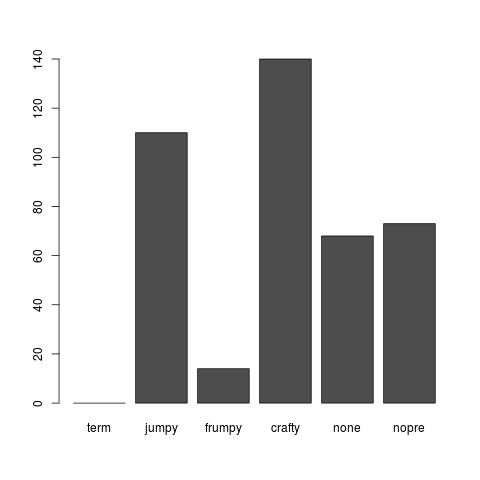
\includegraphics[scale=\figscale]{figures/domsetLabelsE1.png}
	\caption{Distribution of labels of Dominating Set\label{fig:dsLabelsE1}}
\end{figure}
\par Three feature selection methods were used on the dataset all yielding the same result that the feature \inline$normalization$ is the only feature impacting the model significantly. The model was therefore built on this feature as well as on all features available which can be seen in Table~\ref{tbl:feat}.

\par The model on all features had $Precision=0.44$ ($Precision=\frac{tp}{tp+fp}$) and $Recall=0.46$ ($Recall=\frac{tp}{tp+fn}$), yielding $F_1-score=0.45$ ($F_1=2*\frac{precision*recall}{precision+recall}$).
Using only \inline$normalization$ resulted in a slightly worse model having $Precision=0.43$ and $Recall=0.47$, yielding $F_1-score=0.42$. The confusion matrix for both models can be seen in Table~\ref{tbl:dsCME1}. 
\begin{table}[h]
\center
	\begin{tabular}{|c|ccccc|ccccc|}
		\hline
		\multicolumn{6}{|c|}{All Attributes} &\multicolumn{5}{|c|}{normalization}\\
		\hline &$1$&$2$&$3$&$4$&$5$&$1$&$2$&$3$&$4$&$5$\\
		 \hline$1$ & $43$ & $0$ & $38$ & $0$ & $0$ & $61$ & $0$ & $20$ & $0$ & $0$\\
		 $2$ & $2$ & $0$ & $1$ & $0$ & $0$ & $2$ & $0$ & $1$ & $0$ & $0$\\
		 $3$ & $44$ & $0$ & $31$ & $0$ & $0$ & $60$ & $0$& $15$ & $0$ &$0$\\
		 $4$ & $1$ & $0$ & $0$ & $0$ & $0$ &$0$ &$0$&$1$&$0$&$0$\\
		 $5$ & $2$ & $0$& $0$ &$0$&$0$&$2$ &$0$&$0$&$0$&$0$\\
		 \hline
	\end{tabular}
	\caption{Confusion Matrix for Dominating Set}
	\label{tbl:dsCME1}
\end{table}

Both models tend to label instances as \inline$jumpy$, the one with all features does slightly better than the one on only \inline$normalization$ although the feature selection heuristics stated that no other feature but \inline$normalization$ has any impact.

Overall the classifier on all features classified $74$ of $162$ instances correctly while the classifer built only on \inline$normalization$ labeled $76$ correctly. This is not a good result since choosing one of the labels \inline$jumpy$ or \inline$crafty$ randomly would give better results.

\subsubsection{SAT}
The distribution of the labels of the instances can be seen in Figure~\ref{fig:satLabelsE1}. This dataset contains instances which could not be solved in the specified maximum time in the benchmark, even the majority of the instances belongs to that class. 

\begin{figure}[h]
	\center
	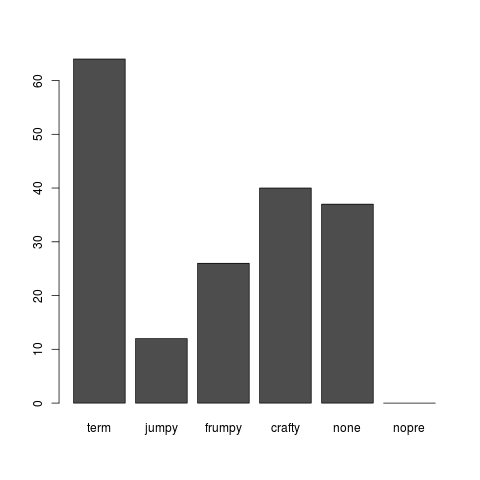
\includegraphics[scale=\figscale]{figures/satLabels.png}
	\caption{Labels of SAT\label{fig:satLabelsE1}}
\end{figure}

Again feature selection methods were used to determine the features with the most impact on the result. Interestingly the heuristics determined \inline$dw$ and \inline$nbredgefacts$ to have big impact, \inline$normalization$ and \inline$defjoin$ to have a little bit of impact and the other features to have very little to no impact on the prediction quality. Therefore models where built using these four features, all features  and only \inline$dw$,\inline$nbredgefacts$.

The model built on all features has $precision=0.32$ and $recall=0.42$, yielding $F_1=0.35$ while the model built on \inline$nomalization$, \inline$dw$, \inline$nbredgefacts$ and \inline$defjoin$ has $precision=0.31$ and $recall=0.41$, yielding $F_1 =0.35$. The classifier built of only \inline$dw$ and \inline$nbredgefacts$ has $precision=0.32$ and recall $F_1=0.42$.

According to the $F_1$ score the model on all features and the model built on only $dw$ and $nbredgefacts$ perform equally, while the model built on the four features predicted best by the feature selection heuristics performs sligthly worse. Looking at the correctly classified instances this effect can be seen too. The models on all features and on \inline$dw$ and \inline$nbredgefacts$ classified $42$ ($42\%$) correctly, while the model on four features classified $41$ ($41\%$) instances correctly. The confusion matrix for the models can be seen in Table~\ref{tbl:satCME1}.

\begin{table}
	\center
	\begin{tabular}{|c|cccccc|cccccc|cccccc|}
		\hline\multicolumn{7}{|c|}{All Attributes} &\multicolumn{6}{|c|}{$4$ attributes}&\multicolumn{6}{|c|}{dw, nbredgefacts}\\
		\hline &$0$&$1$&$2$&$3$&$4$&$5$&$0$&$1$&$2$&$3$&$4$&$5$&$0$&$1$&$2$&$3$&$4$&$5$\\
		\hline $0$ & $4$ & $0$ & $0$ & $2$ & $1$ & $12$& $4$ & $0$ & $0$ & $2$ & $2$ & $11$& $4$ & $0$ & $0$ & $3$ & $2$ & $10$\\
					 $1$ & $1$ & $0$ & $0$ & $0$ & $0$ & $3$ & $1$ & $0$ & $0$ & $0$ & $0$ & $3$ & $1$ & $0$ & $0$ & $0$ & $0$ & $3$\\
					 $2$ & $1$ & $0$ & $0$ & $0$ & $1$ & $2$ & $1$ & $0$ & $0$ & $0$ & $1$ & $2$ & $1$ & $0$ & $0$ & $0$ & $1$ & $2$\\
					 $3$ & $3$ & $0$ & $0$ & $0$ & $2$ & $5$ & $3$ & $0$ & $0$ & $0$ & $2$ & $5$ & $3$ & $0$ & $0$ & $0$ & $2$ & $5$\\
					 $4$ & $4$ & $0$ & $0$ & $0$ & $3$ & $12$& $4$ & $0$ & $0$ & $0$ & $3$ & $12$& $4$ & $0$ & $0$ & $1$ & $3$ & $11$\\
					 $5$ & $4$ & $0$ & $0$ & $0$ & $5$ & $35$& $5$ & $0$ & $0$ & $0$ & $5$ & $34$& $5$ & $0$ & $0$ & $0$ & $4$ & $35$\\
		\hline
	\end{tabular}
	\caption{Confusion Matrix for SAT}
	\label{tbl:satCME1}
\end{table}

\subsubsection{All Instances}
The experiments in this section are the most meaningful since they work with the data from both benchmarks. The input data was obtained by combining the data from both benchmarks.

Again feature selection heuristics were used on the dataset, selecting a subset of $5$ features, \inline$nbredgepred$, \inline$dw$, \inline$nbredgefacts$ and \inline$defjoin$ and \inline$normalization$ as impactful features. Therefore the model was built once on all features, once on the $5$ selected features and once only on \inline$nbredgepred$.

The two model performed equally well regarding the characteristics, having $precision=0.40$ and $recall=0.41$, yielding $F_1=0.39$. Both models were able to classify $40.5\%$ of the instances correctly. The confusion matrix of both models can be seen in Table~\ref{tbl:cmbCM}.

\begin{table}[h]
	\center
	\begin{tabular}{|c|cccccc|cccccc|}
		\hline\multicolumn{7}{|c|}{All Attributes} &\multicolumn{6}{|c|}{$5$ attrib}\\
	\hline &$0$&$1$&$2$&$3$&$4$&$5$&$0$&$1$&$2$&$3$&$4$&$5$\\
\hline$0$&$4$&$1$&$0$&$6$&$1$&$7$&$4$&$0$&$0$&$5$&$1$&$9$\\
$1$&$0$&$38$&$0$&$45$&$0$&$2$&$0$&$35$&$0$&$47$&$0$&$3$\\
$2$&$0$&$3$&$0$&$1$&$1$&$2$&$0$&$3$&$0$&$1$&$2$&$1$\\
$3$&$3$&$46$&$0$&$31$&$0$&$5$&$2$&$46$&$0$&$33$&$0$&$4$\\
$4$&$3$&$4$&$0$&$6$&$3$&$4$&$3$&$3$&$0$&$5$&$4$&$5$\\
$5$&$3$&$6$&$0$&$7$&$0$&$30$&$4$&$6$&$0$&$6$&$0$&$30$\\
\hline
	\end{tabular}
	\caption{Confusion Matrix for all instances}
	\label{tbl:cmbCM}
\end{table}


\subsection{Experiments with \inline$eq$}
For SAT $39$ instances and for Dominating Set no instances were labeled \inline$eq$. We found it interesting to see how labeling instances where all portfolios have the same runtimes with one of the portfolios affects the model. Therefore the same experiments as in the above section were done, labeling instances with equal runtimes with a new label \inline$eq$ instead of labeling them \inline$nopre$. We expected the models to be better using this technique since we thought that labeling all the instances labeled \inline$eq$ with \inline$nopre$ might bias the model.

Surprisingly the models built with label \inline$eq$ performed much worse than the ones without it, not exceeding $precision$ of $0.3$ and $recall$ of $0.35$, and unable to correctly classify most instances. Not more than $35\%$ of the instances were classified correctly in all experiments.

%\subsection{Conclusion}
%While the model for the combined instances does not seem to good considering it only classified $42\%$ of the instances correctly, one should not be disillusioned by it. For most instances the difference in runtimes of the portfolios was only marginally. Therefore classifying an instance wrong wont affect the runtime too much in most cases. 
%Furthermore the model was built on only $505$ instances, it is expected that the quality of the model increases with the size of the learning base.

%It would be interesting to see if the models classify correctly on instances where one of the portfolio was a lot faster than the others but to test this bigger test sets would be needed. Also a classifier built on only those instances could yield interesting results but to get enough data extensive benchmarking would be needed which would break the scope of this project.

